\section{Explanation Factors}
    In this part, we take a look at explanation factors and summarize two different
    methods or standards that are frequently used in recent researches when people start to design or evaluate
    explanations. And an example is also provided in order to illustrate how 
    these methods are used in modern web application.
    \subsection{Seven Explanatory Criterion}

        \indent 
        Like what we have already mentioned in the overview, that the ``seven explanatory criterion''\cite{tintarev2007survey}(see table \ref{table:1}) from Nava Tintarev and Judith Masthoff
        is the most popular standard used to evaluate the explanation. 
        It is comprehensive since it summarized all advantages which explanation can bring to the system. 
        Thus this ``seven explanatory criterion'' will be useful if we want to design explanations.
        \begin{table}[ht] 
            % ht used to attach the table to the position approximately where they are wrote here
            \centering
            \begin{tabular}{ | m{8em} | m{4cm} | }
            \hline
            %  \bfseries used to bold the header
            \bfseries Aim & \bfseries Definition\\ [0.5ex] 
            \hline\hline
            Transparency & Explain how the system works\\ 
            \hline
            Scrutability & Allow users to tell the system it is wrong\\ 
            \hline
            Trust & Increase users' confidence in the system\\ 
            \hline
            Effectiveness & Help users make good decisions\\ 
            \hline
            Persuasiveness & Convince users to try\\ 
            \hline
            Efficiency & Help users make decisions faster\\ 
            \hline
            Satisfaction & Increase the ease of use or enjoyment\\ 
            \hline
            \end{tabular}
            \caption{Explanatory criteria and their definitions}
            \label{table:1}
        \end{table}

        \indent Although they may called differently in different research works
        (``explanation attributes''\cite{al2013explanations}, ``seven possible aims for explanations''\cite{tintarev2012evaluating}
        or ``quality factors''\cite{gedikli2014should}).
        The basic idea is the same,that is to make system more understandable by users.
        
        \indent \textbf{\textit{Transparency:}} Transparency in a recommender system is related to
         the capability of a system to expose the reasoning behind a recommendation to its users\cite{herlocker2000explaining}.
         A recommender systems without explanation works like a ``black box'', which may lost trust from user. 
         Thus, transparency is considered as an important factor to build user's trust in the system\cite{swearingen2002interaction}.

        \indent \textbf{\textit{Scrutability:}} Scrutability means, in short, allow users to tell the system it is wrong.
        It can also be seen as a kind of User Control, which allows users to correct reasoning from system\cite{czarkowski2002scrutable}.
        
        \indent \textbf{\textit{Trust:}} Trust is sometimes linked with transparency.
        Studies have already shown that transparency and 
        the possibility of interaction with recommender systems increases user trust\cite{felfernig2007knowledge}\cite{sinha2002role}.
        
        \indent \textbf{\textit{Effectiveness:}} An effective explanation can help users to make a better decision.
        If an item suggested by the system is the one the user really likes, such explanation can be considered as effective.

        \indent \textbf{\textit{Persuasiveness:}} Persuasiveness, sometimes referred to as promotion, 
        is strongly related to effectiveness and 
        can be defined as the ability of an explanation type to convince the user to accept or disregard certain items\cite{gedikli2014should}.

        \indent \textbf{\textit{Efficiency:}} An explanation is usually considered as efficient when
         it helps the user to decide more quickly or when it helps to reduce the cognitive effort required in the decision process\cite{gedikli2014should}.
         The most common approach to measure it is to look at the iteration time between users and recommender system before users reach their goals.

        \indent \textbf{\textit{Satisfaction:}} The user’s overall satisfaction with a recommender system is assumed to be 
        strongly related to the perceived quality of its recommendations and explanations\cite{swearingen2002interaction}.
 
        \indent What we need to bear in mind, is that, it is hard to design an explanation which
         obeys all seven criterion. In most of the time, we need to have a trade-off. For instance, an explanation that
        offers good transparency may impede efficiency as the user may spend time taking in explanations\cite{tintarev2007survey}.
        In reality, using which criteria depends on the goal of the system. 
    \subsection{Question-type-based Explanation}

    \indent Another possible way to design explanations in context-aware applications is to focus on different question types
    offered by the system. Brian Y. Lim and Anind K. Dey have proposed eight question-type-based explanations\cite{lim2010toolkit}
    This method is quite useful when we intend to design short explanations for automobiles which are mostly used in a context-aware environment.

    These eight question types are:

    \indent \textbf{\textit{Input:}} Explanations inform users which information sources are used to generate the recommendation.

    \indent \textbf{\textit{Output:}} Explanations inform users which output/result is generated by the system.

    \indent \textbf{\textit{What:}} System explains the current state to users (what it is now).

    \indent \textbf{\textit{What If:}} Which results will be generated, if users alter his/her input values(change the behavior).

    \indent \textbf{\textit{Why:}} Explanations inform users why the application derived its output value from the current (or previous) input values\cite{lim2010toolkit}.
    
    \indent \textbf{\textit{Why Not:}} Explanations inform users why another output/result is not chose.
    
    \indent \textbf{\textit{How to:}} Explanations tell users what they can do so that they can get another output/result.

    \indent \textbf{\textit{Certainty:}} Explanations tell users, how certain/uncertain the output/result is.

    In addition to context-aware applications, we can also find some hints of these question types in some other scenarios, like in recommendation systems of e-commercial websites or 
    in some online applications, which are not necessarily ``context-aware''. The next section will show how it may look like in Online Advertisements.
    \subsection{Example -- Explanations in Google Advertisement Recommendation Service}
        As users browse the Internet, read their emails and shop online, they see ads. 
        For example, Google Search results page may show ads similar to a search phrase a user just typed, 
        or user's favorite blog may show interactive ads related to the content on the page.
        These kinds of ads – ads on Google services and millions of websites and apps that partner with Google – are Google ads\cite{googleAdSetting}.
        According this description, we can know that Google Ads is a personalized advertisement service.
        Figure \ref{img:googleAd1} shows an example of Google Ads.
        \begin{figure}[H]
            \centering
            \captionsetup{justification=centering}
            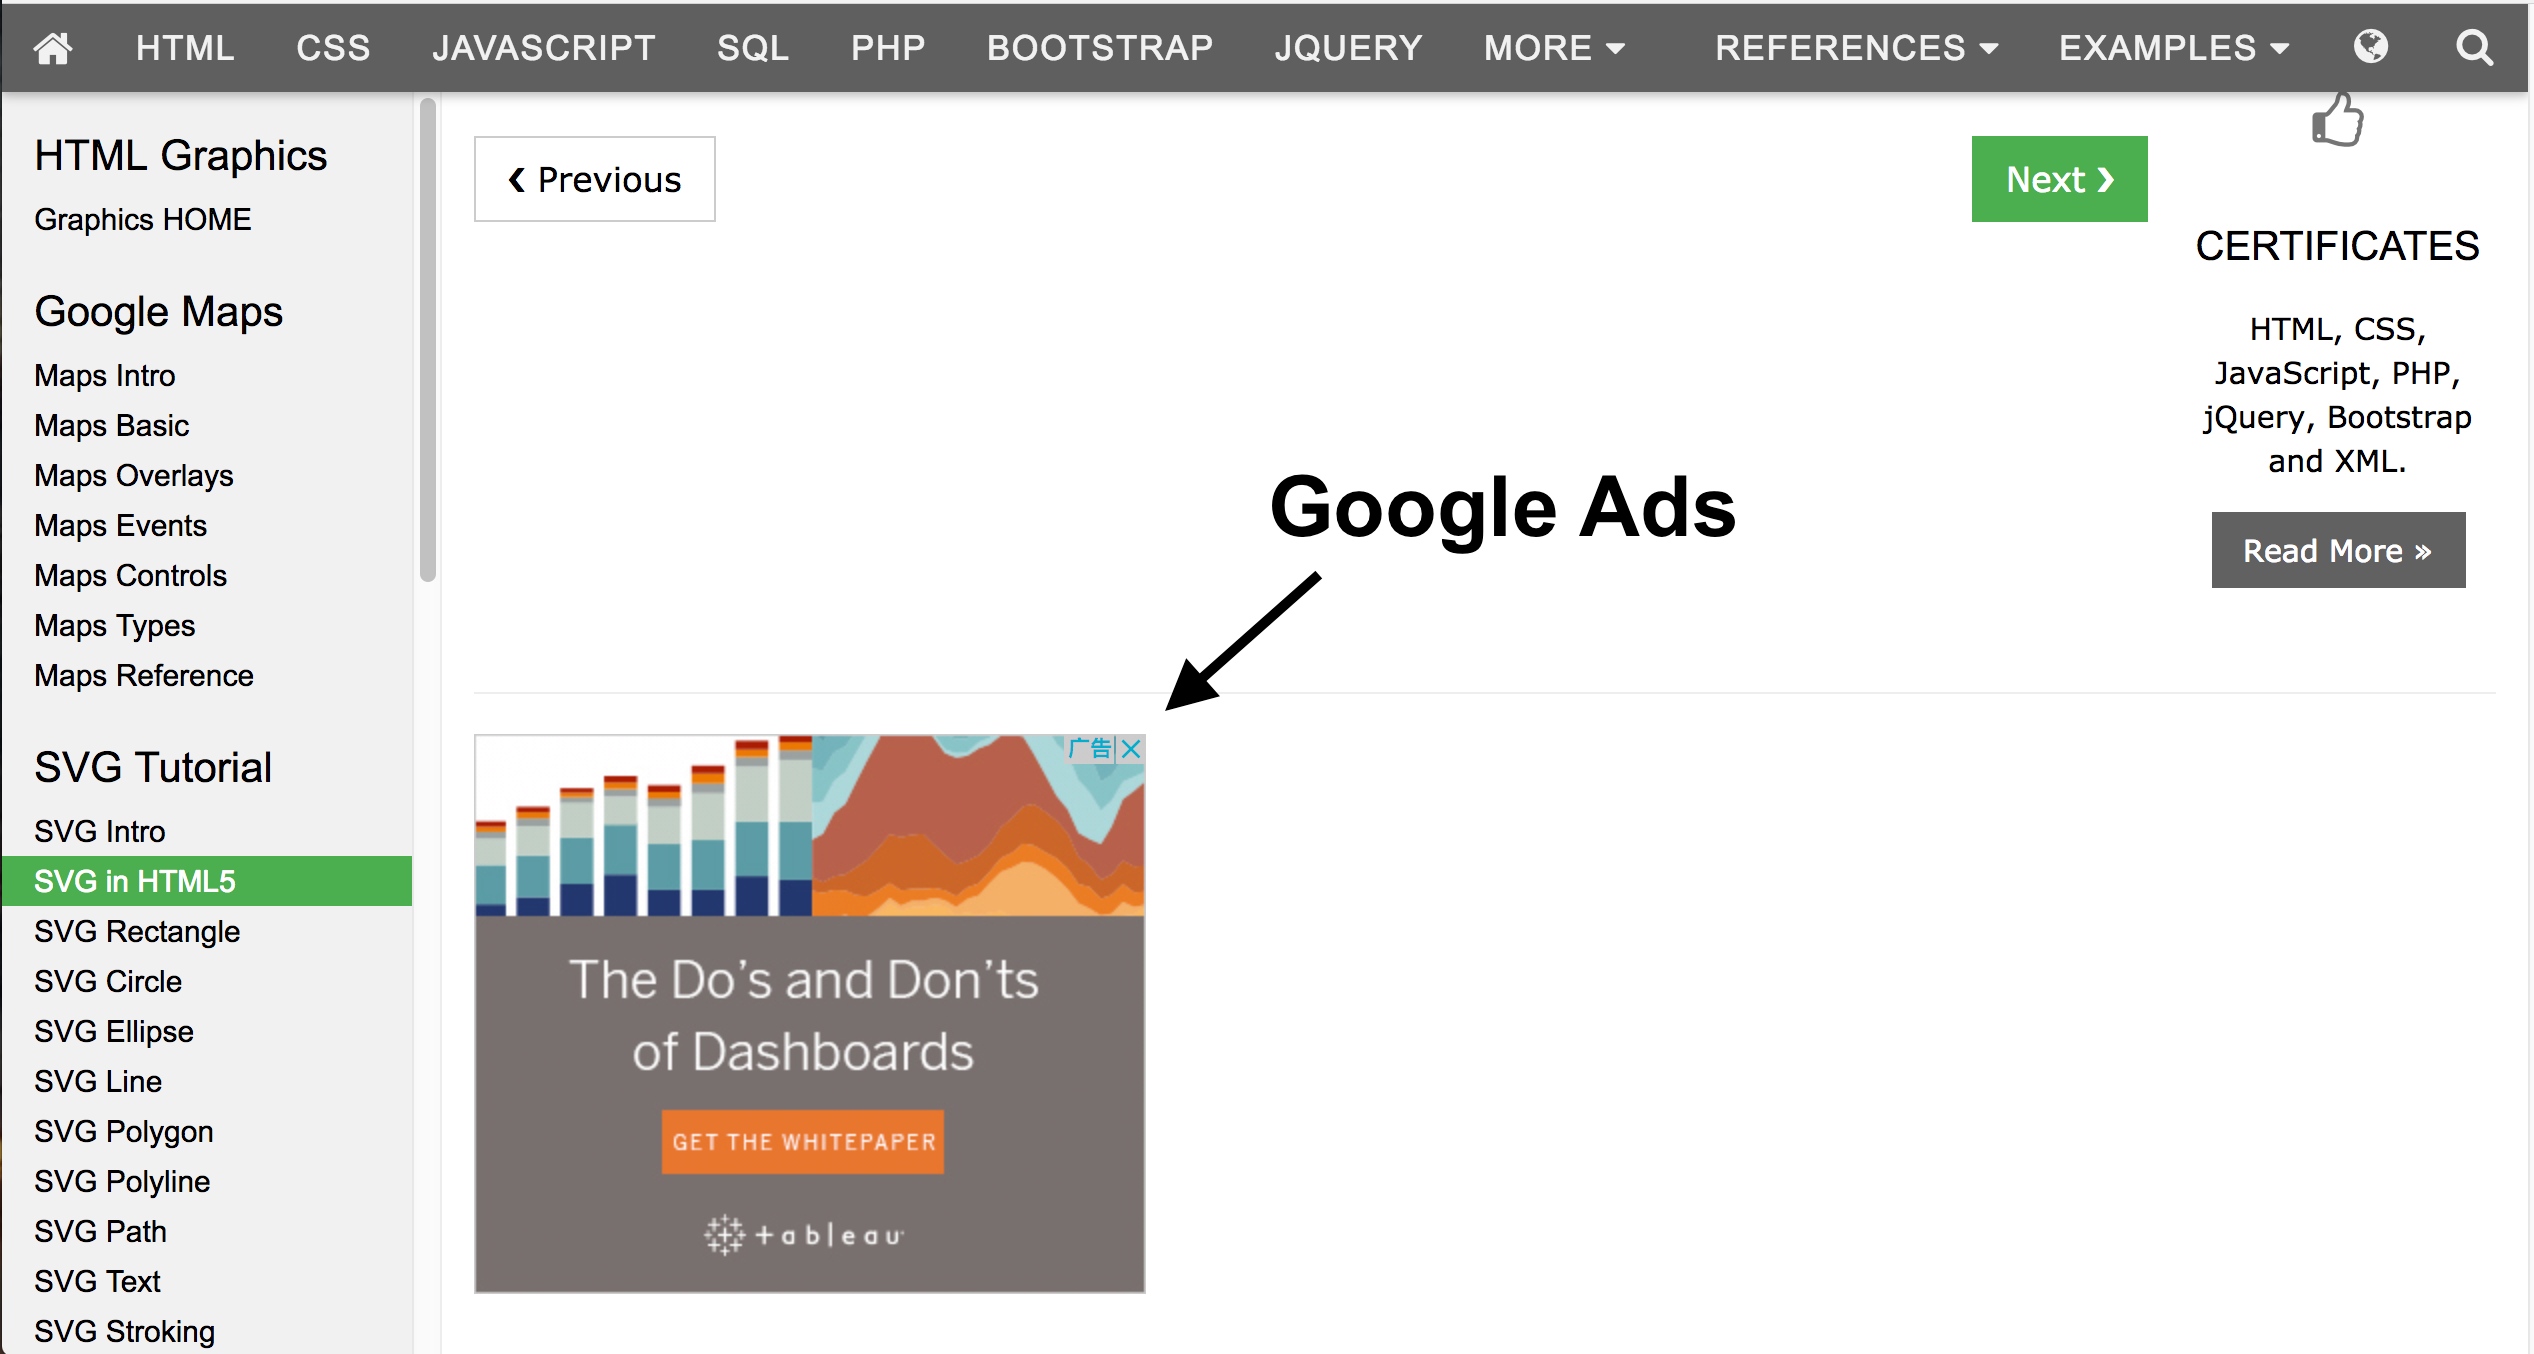
\includegraphics[width=0.5\textwidth]{img/googleAd1}
            \caption{An example of Google Advertisement\cite{googleAd1}}
            \label{img:googleAd1}
        \end{figure}
        \indent Not only the highly personalized service, 
        Google Advertisement also provides users with pages of explanations. 
        We can see here in figure \ref{img:googleAd2}.
        It is the first level of explanations and Google Ads mainly explains two things here.
        ``how does it work'' and ``which information is used''. The first one improves the \textbf{transparency} 
        and increases users' \textbf{trust}, since it exposes the reasoning behind the recommendation to its customers.
       The second one tells users which information Google Ads uses in producing Advertisements. 
       Such information can be seen as a \textbf{Input} type question because it explains 
       users which information sources are used to generate the recommendation.
        \begin{figure}[H]
            \centering
            \captionsetup{justification=centering}
            \begin{mdframed}
                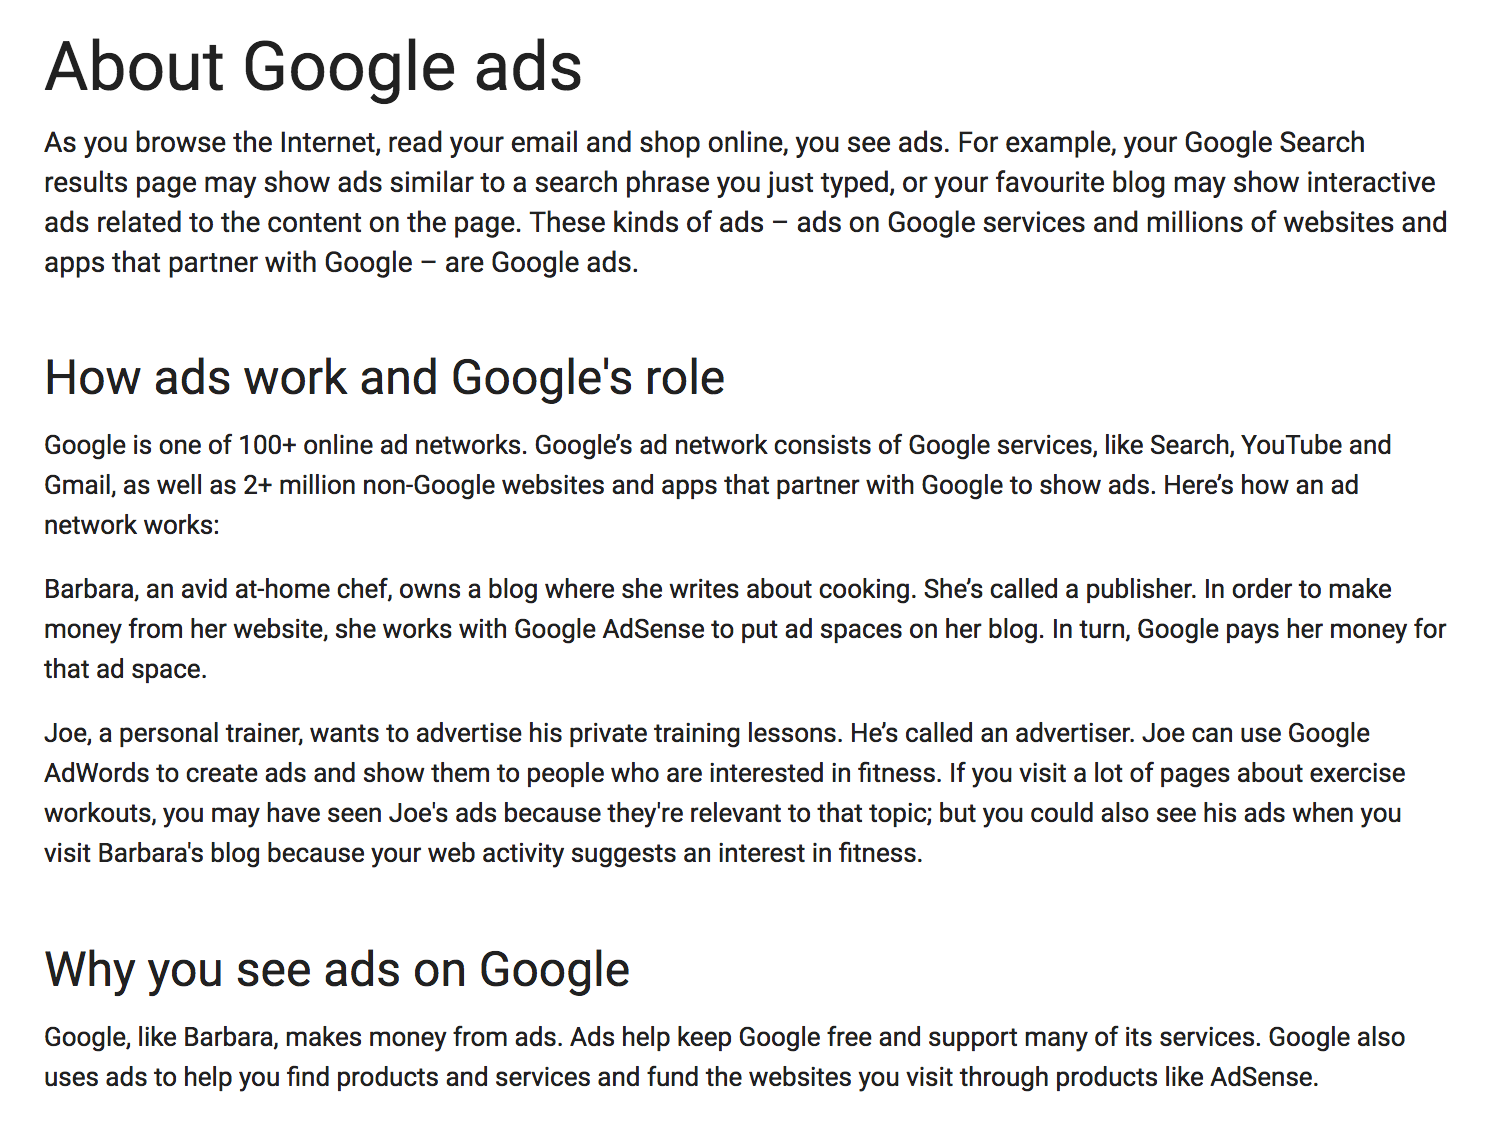
\includegraphics[width=1\textwidth]{img/googleAd2-1}
                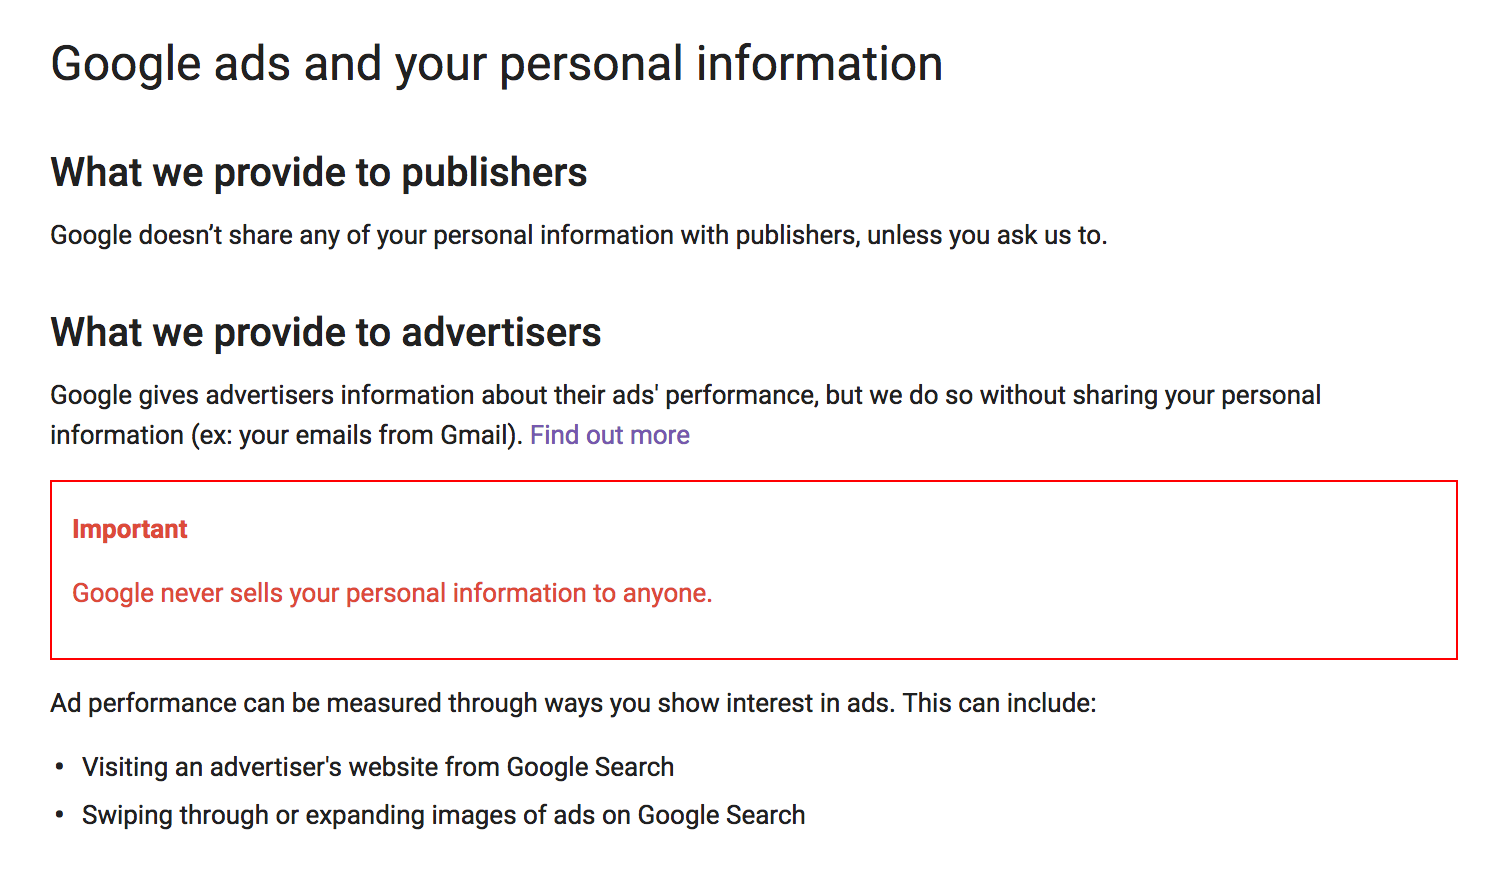
\includegraphics[width=1\textwidth]{img/googleAd2-2}
            \end{mdframed}
            \caption{Explanations from Google Advertisement\cite{googleAd2}}
            \label{img:googleAd2}
        \end{figure}
        \indent Figure \ref{img:googleAd3} shows the second level of explanations in Google Ads.
        It again improves the \textbf{transparency} and increases users' \textbf{trust}. 
        Meanwhile, ``You may see ads on Google Search results pages and other Google services such as Google Maps. 
        The ads you see may be based on what you searched for, your location and the time of day'',
        such information can been seen as a \textbf{Why} 
        and \textbf{Why Not} question types since it explains the reason why users see certain advertisements.
        \begin{figure}[H]
            \centering
            \captionsetup{justification=centering}
            \begin{mdframed}
                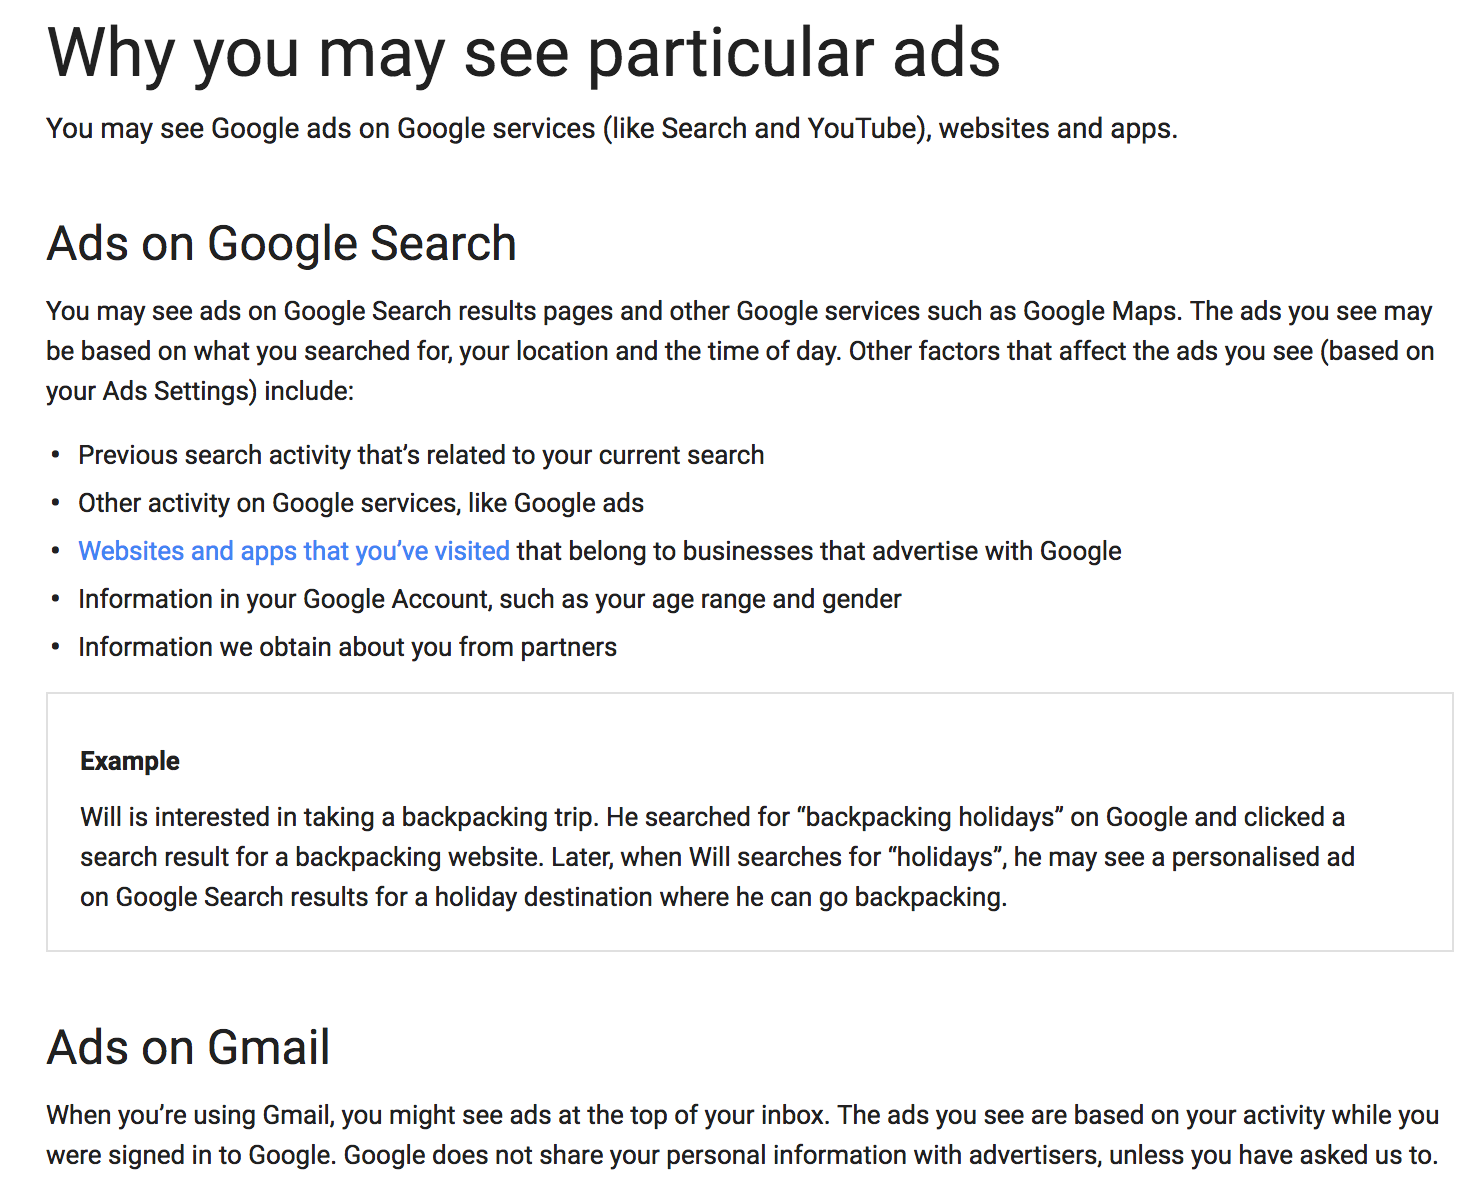
\includegraphics[width=1\textwidth]{img/googleAd3-1}
            \end{mdframed}
            \caption{Explanations from Google Advertisement\cite{googleAd3}}
            \label{img:googleAd3}
        \end{figure}
        In the next level of explanation, it even gives users access to control their personalization.
        In figure \ref{img:googleAd4}, it divides the explanation into users' authority(``What you can do''), 
        users' controls(``Your controls''), users' ability to turn on/off personalization(``Ads Personalization'')
        and how to alter the personalization(``Where your Ads settings apply''). Such accessibility to control
        the personalization can be seen as a symbol of \textbf{Scrutability} since it allows users to avoid the Ads 
        that they are not willing to see. And in the perspective of question-type-based Explanation, it provides users
        with \textbf{What If} and \textbf{How to} type explanations because it teaches users how to alter their personalization.
        \begin{figure}[H]
            \centering
            \captionsetup{justification=centering}
            \begin{mdframed}
                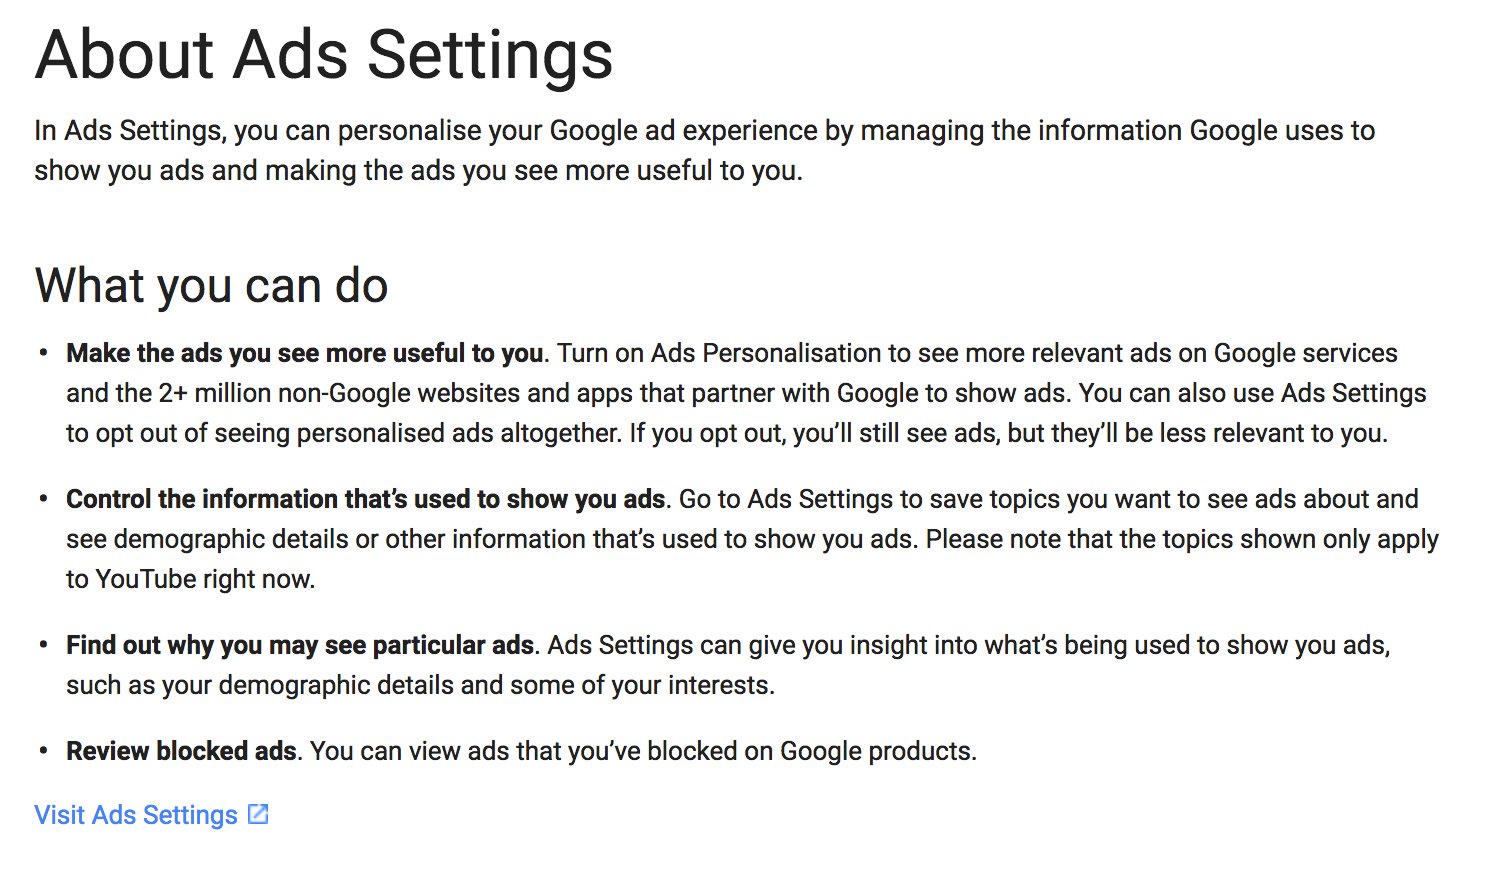
\includegraphics[width=1\textwidth]{img/googleAd4-1}
                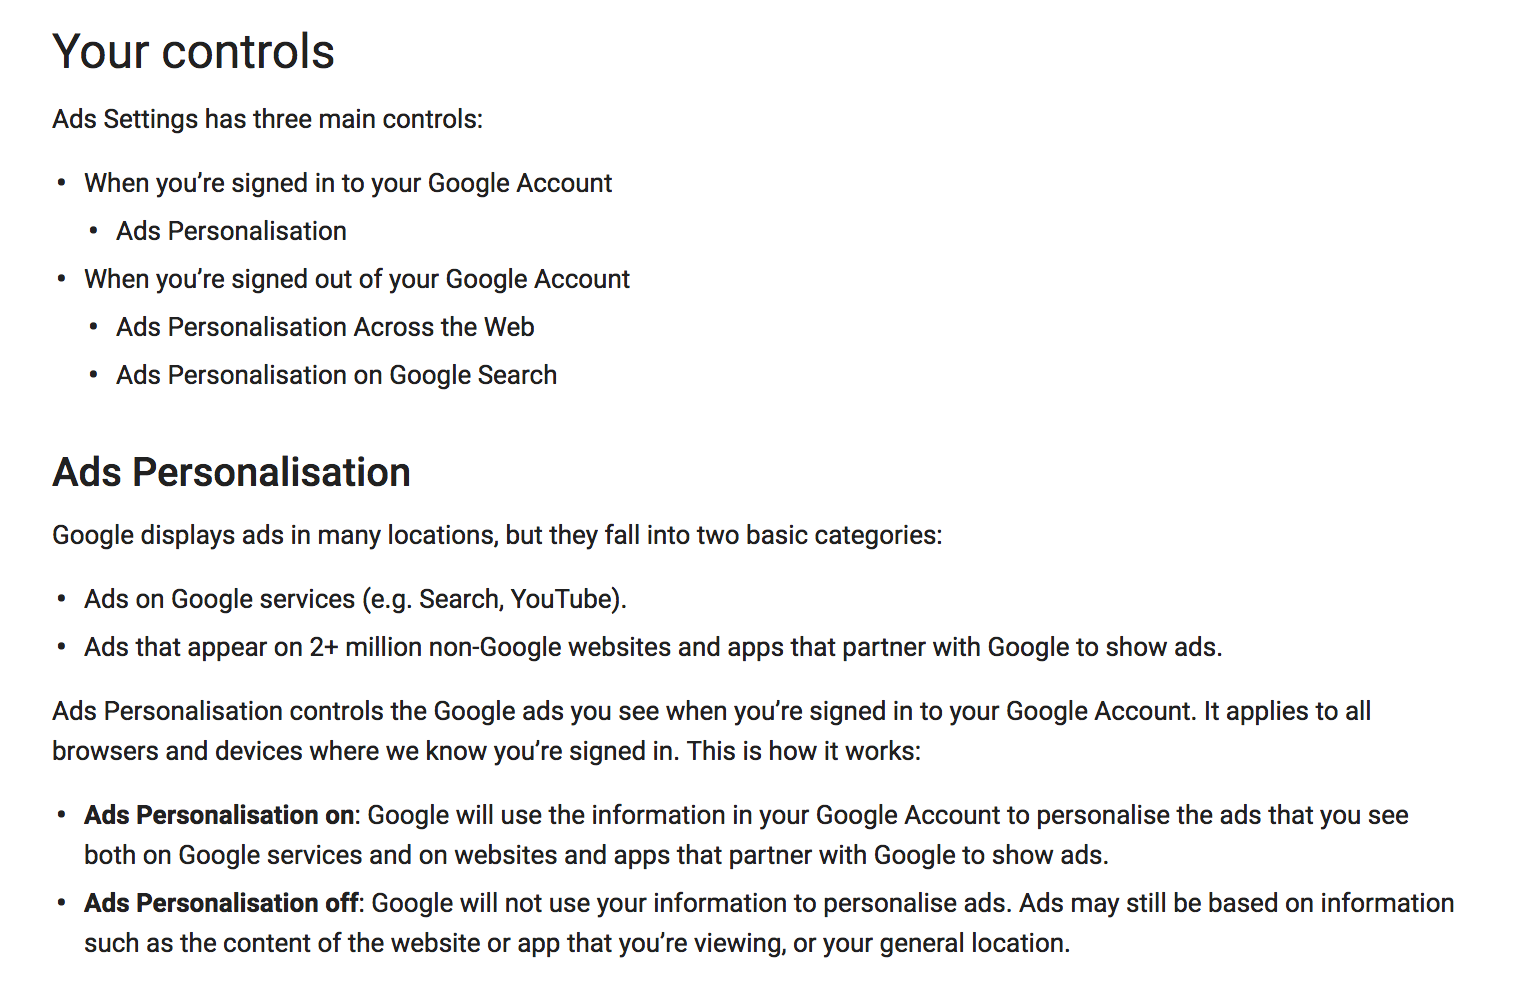
\includegraphics[width=1\textwidth]{img/googleAd4-2}
                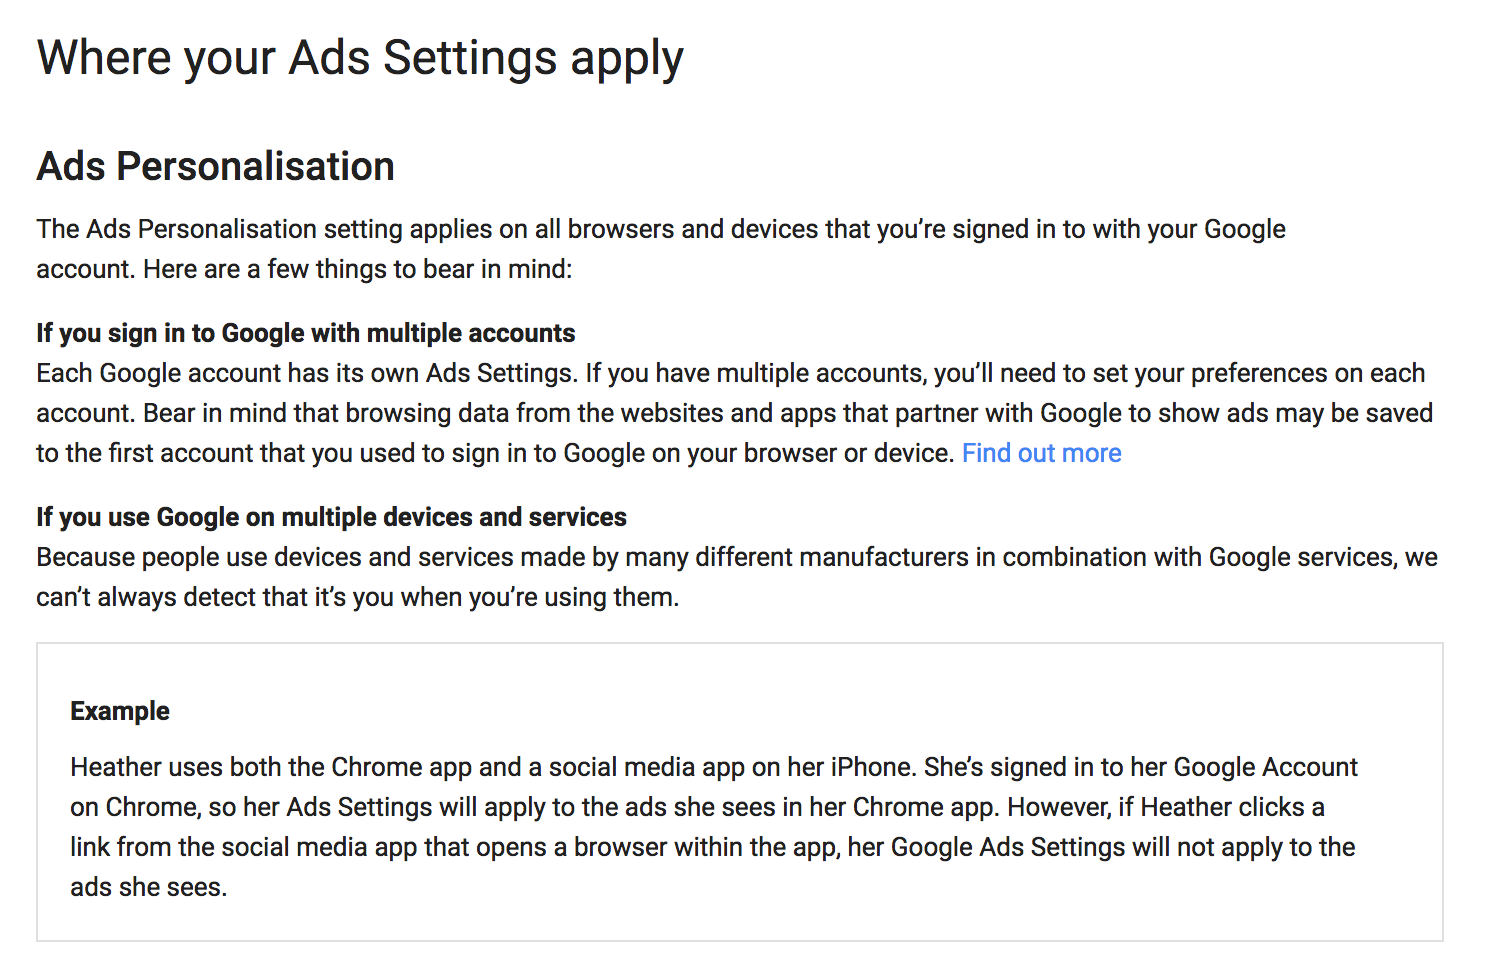
\includegraphics[width=1\textwidth]{img/googleAd4-3}
            \end{mdframed}
            \caption{Explanations from Google Advertisement\cite{googleAd4}}
            \label{img:googleAd4}
        \end{figure}
        Although the explanation from Google Ads is transparent and comprehensive,
        it may not be suitable for some scenarios, like in a driving-context, where short explanation is preferred.
        The next part tries to figure out the connection between two standards(seven explanatory criterion and question-type-based explanation) 
        and short explanations.
\section{Short Explanation}
    In this section, we will dive into short explanation and introduce how this kind of explanations works in a driving-context
    and which criterion or factors are helpful when we try to design short explanation.
    \subsection{Short Explanation related to Seven Explanatory Criterion}
    \indent Like it was already mentioned above, 
    it is recommended to evaluate explanations with seven explanatory criterion. The same works with short explanations.
    Roland Bader and his colleagues have used this criterion and described a method based on knowledge-utility-based 
    recommender systems to extract explanations automatically\cite{bader122011explanations}. They proposed that 
    proactively provided recommendations can reduce driver distraction while searching for information. However, 
    such proactively delivered recommendations may not be accepted by the driver without a suitable explanation.
    Thus their goal was to enhance transparency of proactively delivered recommendations by means of explanations and
    tried to figure out the best way to explain.
    
    \indent They described a gas station recommender of a car and set up a user study with a desktop prototype, 
    in which they provided explanations that were evaluated based on \textbf{efficiency} and \textbf{persuasiveness}.
    Besides what type of explanations should be presented to users, they also wanted to find out how long should an explanation be.
    Thus, they conducted a preliminary study in which they found out that \textbf{two arguments} seemed to be the a good size of explanation
    in the case of gas station(Arguments are like: (1)``this gas station provides gas with very low priced'' or (2)``this gas station is on the route'').
    
    \indent In their user study, explanations are distributed over several levels of detail. 
    The lowest level (first phase) is provided automatically with the recommendations. 
    Then gradually more and more information is accessible by the user manually.
    The elements in the first phase are short explanations for the situation and for the items\cite{bader122011explanations}.
    
    \indent In the phase of evaluation, the first criteria \textbf{persuasiveness} was measured by asking the subjects 
    for their satisfaction with a selection in the first phase and if they need more information. And the second criteria \textbf{efficiency} 
    was measured by looking at how often the subjects needed to switch to deeper phases with more information.

    \indent The result was as expected. Almost all the experimental subjects were satisfied with the first level explanation.
    And they found the information in this stage was adequate for decision-making in normal scenarios, which means that short explanation
    in this case meets the criterion of \textbf{persuasiveness}. The information in second level was selected 
    only if special details were needed, e.g. an ATM or a shop, which means that short explanations in this study in this case meets
    the criterion of \textbf{efficiency}.
    
    \indent In conclusion, it seems that \textbf{persuasiveness} and
    \textbf{efficiency} play a quite important role in short explanation.

    \subsection{Short Explanation related to Question Type}
    
    \indent Another possible approach to design short explanations 
    is to derive explanations from different question types(Why, Why Not, How To, What, What If, Inputs, Outputs and Certainty).
    By Using a driving simulator with an auto-braking function, 
    Martin Steinert and Larry John Leifer have explored how the content of the verbalized message accompanying the car’s autonomous action 
    affects the driver’s attitude and safety performance\cite{koo2015did}.

    \indent Two types of information were provided to explain the auto-braking behavior to the driver during driving(simulated).
    The first one is ``how'' information, which tells the driver the current state of cars(like: ``the car is braking'').
    We need to notice that this kind of explanation equals to \textbf{``what''} question type in Brian's Toolkit\cite{lim2010toolkit}. Thus we will exchange ``how'' to ``what'' in later descriptions. 
    The second one is \textbf{``why''} information, which tells the driver the reason why it behaves in certain ways(like: ``Obstacle ahead.'').  
    
    \indent In their experiment, they employed a two-by-two between-participants experimental design(see table \ref{table:2}).
    In table \ref{table:2}, external information is like ``Obstacle ahead'' while internal information described car activity(``The car is braking'').
    The autonomous action(automatically braking) took place during driving(simulated) and each time, one of the four different types of explanations would be presented:
    \begin{enumerate}
        \item No explanation.
        \item \textbf{``what''} explanation(``The car is braking'') short before the automatically braking.
        \item \textbf{``why''} explanation(``Obstacle ahead'') short after the automatically braking.
        \item A combination of \textbf{``what''} and \textbf{``why''} explanation(``The car is braking due to obstacle ahead'').
    \end{enumerate}
    \begin{table}[ht] 
        % ht used to attach the table to the position approximately where they are wrote here
        \centering
        \begin{tabular}{ | m{2cm} | m{6em} | m{2cm} | }
        \hline
        %  \bfseries used to bold the header
            & \bfseries Why message & \bfseries without Why message\\ [0.5ex] 
        \hline
        \bfseries what message & Both internal and external information referring to automation & Internal (car activity) information\\ 
        \hline
        \bfseries Without what message & External (situation) information & No information (control condition)\\ 
        \hline
        \end{tabular}
        \caption{Structure of study\cite{koo2015did}}
        \label{table:2}
    \end{table}

    \indent Drivers' attitudes and safety performance would be assessed 
    in order to learn how different types of information affect the driver. 
    
    \indent The result showed something different than the original hypothesis.
    A combination of explanation(\textbf{``why''} + \textbf{``how''}) was supposed to 
    improve driving behaviors. However, the result indicated that it affected driver attitude negatively.
    When people were told both how and why the car was about to act on their behalf, they felt anxious.
    According to Martin Steinert and Larry John Leifer. One possible reason for this result
    was that the driver must process two types of information( the machine’s status and the situational status) at the same time,
    which created large cognitive load. Although it was perceived negatively, the combination of explanation
    contributed to safer driving by minimizing off-lane excursions. Thus for further studies, we need to anticipate
    a potential design trade-off between attitudinal preferences and driving safety.

    \indent By only providing \textbf{``how''} explanation, drivers performed the worst: they drifted out of their lane.
    It seems that drivers felt like they took an passive role in driving if they only received \textbf{``how''} explanation.
    Another possible reason is that we human beings expect a polite machine behaviors\cite{reeves1996people}.
    And only explaining the car’s behavior, ``Car is braking,'' without explaining the reason might be “impolite”.
    
    \indent \textbf{``Why''} explanation alone created the least anxiety and highest trust. This kind of behavior from the system
    can be seen as \textbf{transparent}, which can in turn gain more \textbf{trust} from users. 
    Compared with the combination of explanation(\textbf{``why''} + \textbf{``how''}), 
    the amount of time that it takes to hear and cognitively process the why-only message is shorter, 
    which allowed a quicker response/reaction from the driver. Besides, drivers might find the data valuable and credible when the data content satisfies their cognitive need (explain the system behavior).
    For this reason, the \textbf{``why''} explanation is more important to drivers and safer because drivers can anticipate upcoming events\cite{koo2015did}.
